\documentclass[english, 11 pt, class=article, crop=false]{standalone}
%\documentclass[english, 11 pt]{report}
\usepackage[T1]{fontenc}
\usepackage[utf8]{luainputenc}
\usepackage{babel}
\usepackage[hidelinks, bookmarks]{hyperref}
\usepackage{geometry}
\geometry{verbose,tmargin=1cm,bmargin=3cm,lmargin=4cm,rmargin=4cm,headheight=3cm,headsep=1cm,footskip=1cm}
\setlength{\parindent}{0bp}
\usepackage{amsmath}
\usepackage{amssymb}
\usepackage{esint}
\usepackage{import}
\usepackage[subpreambles=false]{standalone}
%\makeatletter
\addto\captionsenglish{\renewcommand{\chaptername}{Kapittel}}
\makeatother
\usepackage{tocloft}
\addto\captionsenglish{\renewcommand{\contentsname}{Innhold}}
\usepackage{graphicx}
\usepackage{placeins}
\raggedbottom
\usepackage{calc}
\usepackage{cancel}
\makeatletter
\usepackage{color}
\definecolor{shadecolor}{rgb}{0.105469, 0.613281, 1}
\usepackage{framed}
\usepackage{wrapfig}
\usepackage{bm}
\usepackage{ntheorem}

\usepackage{ragged2e}
\RaggedRight
\raggedbottom
\frenchspacing

\newcounter{lign}[section]
\newenvironment{lign}[1][]{\Large \refstepcounter{lign} \large
	\textbf{\thelign #1} \rmfamily}{\par\medskip}
\numberwithin{lign}{section}
\numberwithin{equation}{section}
\usepackage{xcolor}
\usepackage{icomma}
\usepackage{mathtools}
\usepackage{lmodern} % load a font with all the characters
\usepackage{xr-hyper}
\makeatother
\usepackage[many]{tcolorbox}

%\setlength{\parskip}{\medskipamount}
\newcommand{\parskiplength}{11pt}
%\setlength{\parskip}{0 pt}
\newcommand\eks[2][]{\begin{tcolorbox}[enhanced jigsaw,boxrule=0.3 mm, arc=0mm,breakable,colback=green!30] {\large \textbf{Eksempel #1} \vspace{\parskiplength}\\} #2 \vspace{1pt} \end{tcolorbox}\vspace{1pt}}

\newcommand\fref[2][]{\hyperref[#2]{\textsl{Figur \ref*{#2}#1}}}
\newcommand{\hr}[2]{\hyperref[#2]{\color{blue}\textsl{#1}}}

\newcommand\rgg[2][]{\begin{tcolorbox}[boxrule=0.3 mm, arc=0mm,colback=orange!55] #2 \vspace{1pt} \end{tcolorbox}\vspace{-2pt}}
\newcommand\alg[1]{\begin{align*} #1 \end{align*}}
\newcommand\algv[1]{\vspace{-11 pt} \begin{align*} #1 \end{align*}}
\newcommand\vs{\vspace{-11 pt}}
\newcommand\g[1]{\begin{center} {\tt #1}  \end{center}}
\newcommand\gv[1]{\begin{center} \vspace{-22 pt} {\tt #1} \vspace{-11 pt} \end{center}}
%\addto\captionsenglish{\renewcommand{\contentsname}{Løsningsforslag tentamen R2 H2015}}

% Farger
\colorlet{shadecolor}{blue!30} 

% Figur
\usepackage{float}
\usepackage{subfig}
\captionsetup[subfigure]{labelformat=empty}
\usepackage{esvect}

\newcommand\sv{\textbf{Svar:} \vspace{5 pt} \\}

%Tableofconents
\renewcommand{\cfttoctitlefont}{\Large\bfseries}
\setlength{\cftsubsecindent}{2 cm}
\newcommand\tocskip{6 pt}
\setlength{\cftaftertoctitleskip}{30 pt}
\setlength{\cftbeforesecskip}{\tocskip}
%\setlength{\cftbeforesubsecskip}{\tocskip}

%Footnote:
\usepackage[bottom, hang, flushmargin]{footmisc}
\usepackage{perpage} 
\MakePerPage{footnote}
\addtolength{\footnotesep}{2mm}
\renewcommand{\thefootnote}{\arabic{footnote}}
\renewcommand\footnoterule{\rule{\linewidth}{0.4pt}}

%asin, atan, acos
\DeclareMathOperator{\atan}{atan}
\DeclareMathOperator{\acos}{acos}
\DeclareMathOperator{\asin}{asin}

%Tabell
\addto\captionsenglish{\renewcommand{\tablename}{Figur}}

% Figur
\usepackage[font=footnotesize,labelfont=sl]{caption}
\addto\captionsenglish{\renewcommand{\figurename}{Figur}}

% Figurer
\newcommand\scr[1]{/home/sindre/R/scr/#1}
\newcommand\asym[1]{/home/sindre/R/asymptote/#1}

%Toc for seksjoner
\newcommand\tsec[1]{\phantomsection\addcontentsline{toc}{section}{#1}
	\section*{#1}}
%\newcommand\tssec[1]{\subsection*{#1}\addcontentsline{toc}{subsection}{#1}}
\newcommand\tssec[1]{\subsection*{#1}}
% GeoGebra
\newcommand{\cms}[2]{{\tt #1( #2 )}}
\newcommand{\cm}[2]{{\large \tt #1( #2 )} \gvs \\}
\newcommand{\cmc}[2]{{\large \tt #1( #2 )} \large (CAS)  \gvs \\ \normalsize}
\newcommand{\cmk}[2]{{\large \tt #1( #2 )} \large (Inntastingsfelt)  \gvs \\ \normalsize}

\newcommand\gvs{\vspace{11 pt}}

\newcommand\vsk{\vspace{11 pt}}
\newcommand{\merk}{\vsk \textsl{Merk}: }
\newcommand{\fig}[1]{
\begin{figure}
	\centering
	\includegraphics[scale=0.5]{fig/#1}
\end{figure}
}
\newcommand{\figc}[1]{
		\centering
		\includegraphics[scale=0.5]{fig/#1}
}

% Opg
%\newcommand{\opgt}{\phantomsection \addcontentsline{toc}{section}{Oppgaver} \section*{Oppgaver for kapittel \thechapter}}
\newcounter{opg}
\numberwithin{opg}{section}

\newcommand{\opl}[1]{\vspace{15pt} \refstepcounter{opg} \textbf{\theopg} \vspace{2 pt} \label{#1} \\}



\begin{document}
\eqlen
\opgt
\setcounter{section}{1}
\opl{veiformel2}
I fysikken sier man at når et legeme er i fritt fall, er tyngdekraften den eneste kraften som utfører et arbeid på legemet. Hvis vi innfører en $ y $-akse med positiv retning rett opp, vil tyndeakselerasjonen $ g $ virke i negativ retning. Akselerasjonen $ a $ på legemet kan vi derfor skrive som
	\[ a = -g \]
	Vi lar videre $ y(t) $ betegne legemets posisjon til enhver tid $ t $. Vi kan da skrive farten som $ y' $ og akselerasjonen som $ y'' $. Altså har vi at
	\[ y''=-g \tag{I}\label{opgv0} \]
	\textbf{a)} Finn dene generelle løsningen av (\ref{opgv0}).\os
	
	\textbf{b)} Ofte kaller man startfarten til et legeme for $ v_0 $. Finn løsningen til (\ref{opgv0}) når du vet at $ {y(0)=0} $ og $ {y'(0)=v_0} $.
	
	\nes
	\opl{kjernederye}
	Vis at vi for enhver funksjon $ f(x) $ har at
	\[ \left(y(x) e^{F(x)}\right)' = y'(x)e^{F(x)}+f(x)y(x)e^{F(x)} \]
	hvor $ F $ er en antiderivert til $ f $.
	
	\opl{FODE}
	Løs ligningen:\os
	
	\begin{tabular}{@{}l l }
		\textbf{a)} $ y'+4y=8 $	\quad
		&\textbf{b)} $\displaystyle y' + \frac{1}{x}y - \cos x=0$  \\[11 pt]
		\textbf{c)} $\displaystyle y' + \frac{3}{x}y = 6x +2 $		
		&\textbf{d)} $\displaystyle y'+3x^2 y =(1+3x^2)e^x$ 
	\end{tabular}

\nes	
\opl{sepode}
Finn den generelle løsningen av ligningen:\os

\begin{tabular}{@{}l l l}	
	\textbf{a)} $\displaystyle y'=ye^x \cos x$\quad	
	\textbf{b)} $\displaystyle y'=\frac{1}{y}3x^2(y^2+1) $ 	
\end{tabular}

\opl{sepode2}
Løs ligningen:\os

\textbf{a)} $\displaystyle xy'-y=2x^2y\quad,\quad y(1)=1$\os
\textbf{b)} $2\sqrt{x}y'=\cos^2 y\quad,\quad y(4)=\frac{\pi}{4}$ 
\newpage
\nes
\opl{retnopg}
Figuren under viser et retningsdiagram for en differensialligning.
\begin{figure}
	\centering
	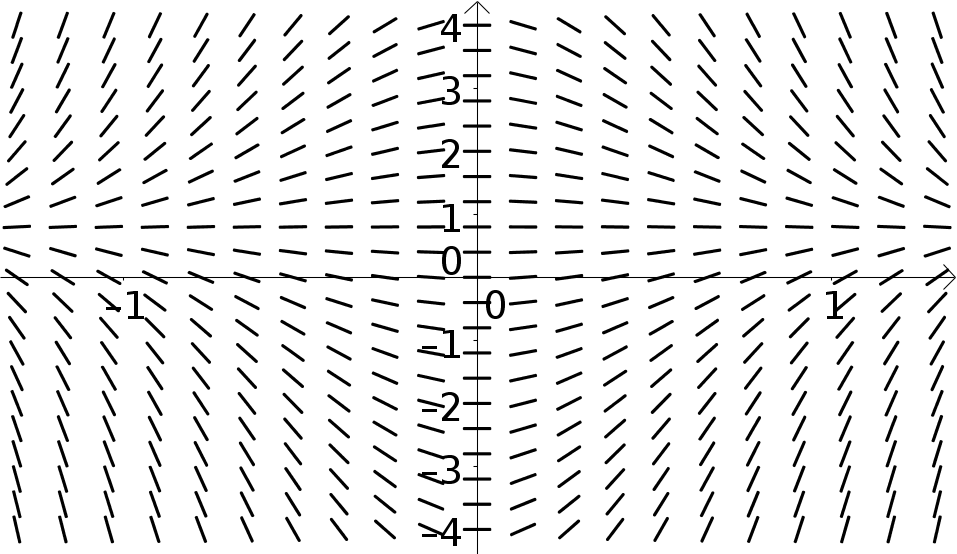
\includegraphics[scale=0.85]{retn}
\end{figure}
\textbf{a)} Skisser integralkurven som går gjennom punket $ (0, 4) $ og integralkurven som går gjennom punktet $ (0, -4) $.\os

\textbf{b)} Bruk figuren til å anslå stigningstallet til alle integralkurvene for $ x=0 $.\vsk

Integralkurvene er løsninger av ligningen $ y' + 4x y = 3x$. 
\os
\textbf{c)} Bruk ligningen til å verifisere anslaget fra oppgave b).\os

\textbf{b)} Finn stigningstallet i punktene $ (-3, 5) $ og $ (4, 2) $.

\nes
\opl{SODEopg}
Finn den generelle løsningen av ligningen:\os

\textbf{a)} $ y''-y'-2y =0 $\os

\textbf{b)} $ 2y''-12y'+18y=0 $\os

\textbf{c)} $ y''-4y'+13y=0 $

\opl{speslos}
Finn løsningen av differensialligningen:\os

\textbf{a)} $ y''-2y'-15y=0\quad,\quad y(0)=-1,\,y'(0)=2 $\os

\textbf{b)} $ y''+10y'+25y=0\quad,\quad y(0)=2,\,y'(0)=1  $\os

\textbf{c)} $ y''-2y'+5y=0\quad,\quad y(0)=1,\,y'(0)=1  $

\nes
\opl{folketall}
I året 2015 var tallet på en populasjon 100 millioner. Fra og med dette året er det forventet at folkeveksten vil være proporsjonal med folketallet.\os

\textbf{a)} Sett opp en differensialligning som beskriver situasjonen over.\os

\textbf{b)} I 2016 var folketallet 101 millioner. Bruk denne informasjonen til å finne uttrykket $ y(t) $ som gir folketallet (i millioner) $ t $ år etter 2015.

\opl{newtavkj}
En gjenstand med temperaturen $ T$ befinner seg i et rom med temperaturen $ T_r $. Det antas at temperaturen til gjenstanden er likt fordelt hele tiden og at romtemperaturen ikke blir påvirket av gjenstandens temperatur. Når $ T$ er høyere enn $ T_r $ kan vi bruke \textit{Newtons avkjølingslov} for å tilnærme hvordan $ T $ vil utvikle seg med tiden $ t $:
\[ T'=-k(T-T_r) \]
$ k $ er en konstant som må bestemmes ut ifra gjenstandens termodynamiske egenskaper. \os

\textbf{a)} Finn den generelle løsningen av ligningen over.

En gjenstand med temperaturen 95\,$ ^\circ $C blir plassert i et rom med temperaturen 15\,$ ^\circ $C. Vi bruker Newtons avkjølingslov til å anslå gjenstandens temperatur $ T $ etter $ t $ minutter. $ k $ har verdien $ \frac{\ln 2}{5} $. \os

\textbf{b)} Finn et uttrykk for $ T $.\os

\textbf{c)} Bestem $ T(15) $.\os

\textbf{d)} Hva skjer når vi lar tiden gå mot uendelig?

\opl{fjormassopg}
Gitt en funksjon $ y(t) $ på formen
\[y(t) =a\cos (\omega t) +b\sin (\omega t) \] 
hvor $ a $, $ b $ og $ \omega $ er konstanter (når $ t $ er en tidsvariabel, kaller vi gjerne $ \omega $ for \textit{vinkelfrekvensen}\index{vinkel!-frekvens}). Vis at vi for alle fjør-masse systemer uten demping har at
\[ \omega=\sqrt{\frac{k}{m}} \] 

\opl{demfjoropg}
En klosse med masse $ {m=1} $ henger vertikalt i en fjør med fjørkonstant $ {k=25} $. Klossen strekkes slik at den forflyttes en lengde $ 0.5 $ fra likevektspunktet $ {y=0} $, og blir etterpå sluppet. La $ y(t) $ være forflytningen relativt til likevektspunktet tiden $ t $ etter at bevegelsen har startet.\os

\textbf{a)} Finn et uttrykk for $ y $.\os

\textbf{b)} Finn perioden til $ y $.

Klossen og fjøren blir plassert i en omgivelse der dempingskonstanten er funnet å være $ {q=6} $. Ved et tidspunkt satt til $ {t=0} $ passerer klossen likevektspunktet med en fart $ y'(0)=4 $.\os

\textbf{c)} Finn det nye uttrykket for $ y $. 

\ekspop
\textbf{a)} Vis at vi kan omskrive et fjør-masse system med demping til ligningen
\[ y''+2\alpha y'+\omega^2y=0 \tag{I}\label{kritisk} \]
hvor $ 2\alpha=\frac{b}{m} $ og $ \omega=\sqrt{\frac{k}{m}} $.\os

\textbf{b)} Vis at løsningen av den karakteristiske ligningen av (\ref{kritisk}) kan skrives som
\[ r=-\alpha\pm\sqrt{\alpha^2-\omega^2} \]
\textbf{c)} For de tre tilfellene $ \alpha>\omega $, $ \alpha=\omega $ og $ \alpha<\omega $, hvilket uttrykk antar løsningen av (\ref{kritisk})? \os

\textsl{Hint}: Se (\ref{tore})-(\ref{kompleks}).\os%(Oppgaven fortsetter på neste side).

\textbf{d)} La $ y(t) $ være løsningen av (\ref{kritisk}). Forklar hvorfor $ \lim\limits_{t\to\infty}y(t) =0 $. (Ta det for gitt at $ \lim\limits_{t\to \infty} te^{-at}=0 $ når $ a>0 $).
\end{document}